\section{Preliminaries}\label{sec:prel}

\subsection{Multisignatures}\label{sec:multisig}
%\label{sec:prel_ms}
%
% At the current stage of this document, the formal security definition
% of \emph{multisignatures (MS)} is omitted in favor of an intuitive
% understanding of their security.  More details can be found in
% \cite[Section 4.1]{sidechains}.
A multisignature scheme~\cite{itakura1983public,CCS:MicOhtRey01} is a
tuple of algorithms:

\vspace{5mm}$\ms = (\msSetup \times \allowbreak\msKeyGen \times \allowbreak\msCombVK \times \allowbreak
\msSign \times \allowbreak\msComb \times \allowbreak\msVfy)$
\vspace{5mm}\\*such that
$\msParams \gets \msSetup(1^\spara)$ generates public parameters;
%$\msParams$;
% with security parameter $k$;
\\*with these in place,
$(\msVK,\msSK) \gets \msKeyGen(\msParams)$ can be used to generate
fresh key pairs. 
\vspace{5mm}\\*Then
%Signatures are managed with the remaining algorithms:
\begin{mitemize}
%\hspace{5mm}begin{enumerate*}[label=(\roman*)]
  \item $\msSig \gets \msSign(\msParams,\msSK,\msMsg)$ signs 
    a message $\msMsg$ using key $\msSK$;
  \item $\msCSig \gets \msComb(\msParams,\msMsg,\msVKL,\msSigL)$ aggregates a
    set $\msSigL$ of signatures into a single, aggregate signature~$\msCSig$.
  \end{mitemize}
  The algorithm $\msCVK \gets \msCombVK(\msParams,\msVKL)$ aggregates
  a tuple $\msVKL$ of verification keys $\msVK$ into a single,
  aggregate verification key $\msCVK$ which can be used for verification:
  %to verifiy an  aggregated signature:
  $\msVfy(\msParams,\msCVK,\msMsg,\msCSig) \in \{\true,\false\}$
  verifies an aggregate signature under an aggregate verification key.
  In the following, we often make the parameter~$\msParams$ implicit in the
    function calls for better readability.

  Intuitively, the security of a multisignature scheme guarantees
  that, if $\msCVK$ is produced from a tuple of verification keys
  $\msVKL$ via $\msCombVK$, then no aggregate signature $\msCSig$ can
  pass verification $\msVfy(\msCVK,\msMsg,\msCSig)$ unless all
  honest parties holding keys in $\msVKL$ signed $m$.

\subsection{Extended UTxO model \& state machines}
\label{sec:prel_tx}

The basis for our fast isomorphic state channels is Bitcoin's UTxO ledger model~\cite{formal-model-of-bitcoin-transactions,Zahnentferner18-UTxO}. It arranges transactions in a directed acyclic graph structure, thus making the available parallelism explicit: any two transactions that are not directly or indirectly dependent on each other can be processed independently. 

\begin{figure}[t]
  \centering
  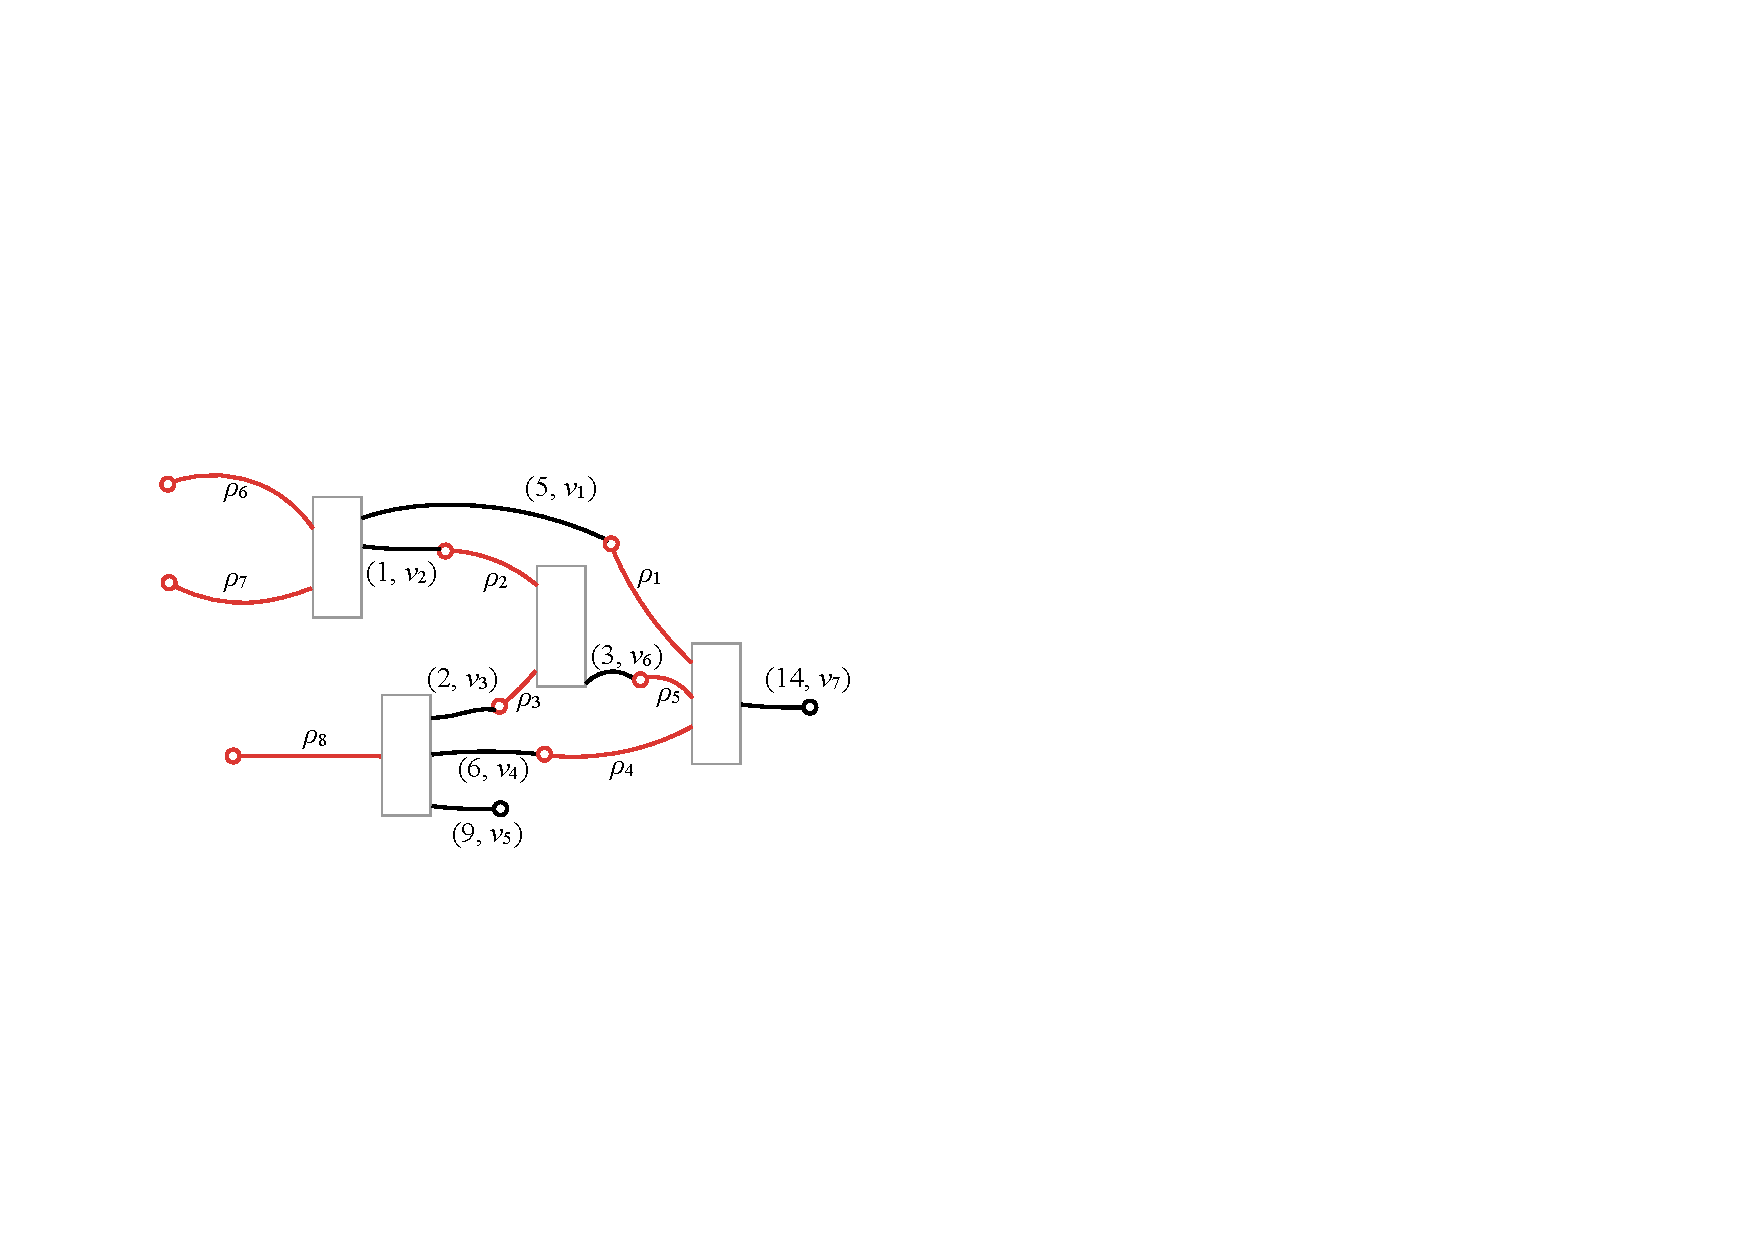
\includegraphics[scale=.2,width=\textwidth/2]{figures/utxo-graph.pdf}
  \caption{Example of a plain UTxO graph}
  \label{fig:utxo-graph}
\end{figure}
%
\dparagraph{UTxO.}
Transactions in an UTxO ledger contain a set of inputs and outputs, where outputs lock an amount of cryptocurrency, such that only authorized inputs of subsequent transactions can connect and consume those funds. This arrangement results in graphs, such as the one in Figure~\ref{fig:utxo-graph}, where the boxes represent transactions with (red) inputs to the left and (black) outputs to the right.

Each output locks some cryptocurrency, which can be transferred via a subsequent transaction by consuming that output with a new input. The set of dangling (unconnected) outputs are the \emph{unspent transaction outputs (UTxOs)} --- there are two of those in Figure~\ref{fig:utxo-graph}. In addition to the locked currency, each output also comes with a predicate $\nu$, called its \emph{validator}. In Figure~\ref{fig:utxo-graph}, we use pairs \((n, \nu)\) to indicate that a given output locks $n$ cryptocurrency with validator predicate $\nu$.

Where outputs carry validators, each input comes with a \emph{redeemer} value $\rho$. To determine whether a given input of the currently validated transaction $\txTx$ is permitted to connect to a, as of yet, unspent output, we determine whether the validator predicate $\nu$ of that output applies for the redeemer $\rho$; or more formally, we check that \(\nu(\rho, \sigma) = \true\), where the \emph{validation context} $\sigma$ represents some properties of the transaction that the spending input belongs to, such as the transaction's cryptographic hash value. For example, the validator may require the redeemer to be a signature on the transaction hash contained in the context $\sigma$ for a specific key pair, such that only the owner of the private key can spend an output locked by that validator.

\dparagraph{Extended UTxO.}
%\label{sec:eutxo}
The \emph{Extended UTxO Model (EUTxO)}~\cite{eutxo} preserves this
structure, while adding support for more expressive smart contracts
and, in particular, for multi-transaction state machines, which serve
as the basis for the mainchain portion of the work presented
here. This additional expressiveness is achieved by two changes to the plain UTxO scheme outlined before: 
%
\begin{itemize}
\item Outputs carry, in addition to a cryptocurrency value $n$ and a validator $\nu$, now also a \emph{datum} $\delta$, which can, among other things, be used to maintain the state of long running smart contracts.
\item The validation context $\sigma$ is extended to contain the entire validated transaction $\txTx$ as well as the UTxOs consumed by the inputs of that transaction.
\end{itemize}
%
In this extended model, evaluation of the validator predicate implies checking \(\nu(\rho, \delta, \sigma) = \true\). Besides maintaining contract state in $\delta$, the fact that the validator can inspect the entire validated transaction $\txTx$ through $\sigma$ enables validators to enforce that contract invariants are maintained across entire chains of transactions.

Although formal results about EUTxO are rather recent, extended UTxO models already form the basis for the smart-contract platforms of existing blockchains --- in particular, Cardano~\cite{plutus-platform} and Ergo~\cite{ergo-platform}. Consequently, the Hydra head protocol as presented in this paper is of immediate practical relevance to these existing systems.

\dparagraph{User-defined tokens.}
%
In addition to the basic EUTxO extension, we generalize the
currency \emph{values} recorded on the ledger from integral numbers to \emph{generalized
  user-defined tokens}~\cite{eutxo-2}.
%\footnote{As per the EUTXO-2 model defined in
%\url{https://github.com/hydra-supplementary-material/eutxo-spec/blob/master/extended-utxo-specification.pdf}}
% \footnote{As per the EUTXO-2 model defined in
% \url{https://github.com/input-output-hk/plutus/tree/master/extended-utxo-spec}}
Put simply (sufficient to understand the concepts in this paper),
values are sets that keep track how many units of which tokens of
which currency are available.  For example, the value
$\{\mathsf{Coin} \mapsto \{\mathsf{Coin} \mapsto 3\}, c \mapsto \{t_1
\mapsto 1, t_2 \mapsto 1\}\}$ contains $3$ $\mathsf{Coin}$ coins
(there is only one (fungible) token $\mathsf{Coin}$ for a payment
currency $\mathsf{Coin}$), as well as (non-fungible) tokens $t_1$ and $t_2$, which
are both of currency $c$.  Values can be added naturally, e.g.,
\begin{align*}
  & \{\mathsf{Coin} \mapsto \{\mathsf{Coin} \mapsto 3\}, c \mapsto \{t_1
    \mapsto 1, t_2 \mapsto 1\}\} \\
  + \ & \{\mathsf{Coin} \mapsto \{\mathsf{Coin} \mapsto 1\}, c \mapsto \{t_3 \mapsto 1\}\} \\
  = \ & \{\mathsf{Coin} \mapsto \{\mathsf{Coin} \mapsto 4\}, c \mapsto \{t_1
        \mapsto 1, t_2 \mapsto 1, t_3 \mapsto 1\}\} \ .
\end{align*}
%
In the following, $\varnothing$ is the empty value, and
\(\{t_1, \ldots, t_n\} :: c\) is used as a shorthand for
\(\{c \mapsto \{t_1 \mapsto 1, \ldots, t_n \mapsto 1\}\}\).



% \begin{definition}[Values]
%   Values \(\txVal : \txValTy\) are finitely-supported functions
%   \(\txCIdTy \mapsto \txTokenTy \mapsto {\mathbb{Z}}\) (where
%   \emph{currency identifiers} $\txCIdTy$ and tokens $\txTokenTy$ are
%   cryptographic hashes). Values form monoids with $+$ as the
%   combining operation, and we write $\emptyset$ for the neutral
%   element (i.e., no value).  We write
%   \(\txVal\setminus\{t_1, \ldots, t_n\}\) to denote $\txVal$ where
%   all tokens \(t_1, \ldots, t_n\) have been removed.

%   Given a value that contains multiple tokens $t_1$, \ldots $t_n$
%   with quantity $1$, all of which belong to the same currency
%   identifier $c$, we write \(\{t_1, \ldots, t_n\} :: c\) as a
%   shorthand for the full map
%   \(\{c \mapsto \{t_1 \mapsto 1, \ldots, t_n \mapsto 1\}\}\).  If it
%   is clear from the context, we may omit the currency identifier $c$
%   and simply write \(\{t_1, \ldots, t_n\}\).
% \end{definition}

The EUTxO ledger consists of \emph{transactions}: Transactions are
quintuples $\tx = (I,O,\txValForge,r,\txKeys)$ comprising a set of
\emph{inputs} $I$, a list of \emph{outputs} $O$, values of
\emph{forged/burned tokens} $\txValForge$, a \emph{slot range}
\(r = (\txRmin, \txRmax)\), and a set of public keys $\txKeys$.
%
Each input \(i\in I\) is a pair consisting of an \emph{output
  reference} $\txOutRef$ (consisting of a transaction ID and an index
identifying an output in the transaction) and a \emph{redeemer} $\rho$
(used to supply data
% used
for validation).
% 
Each output \(o\in O\)
is % either (1) a pair \((\txVal, \kappa)\) of a
% value $\txVal$ and a public key $\kappa$ (\emph{pubkey output}) or
% (2)
a triple \((\txVal, \nu, \delta)\) consisting of a value $\txVal$, a
validator script $\nu$, and a datum
$\delta$. % (\emph{script output}).
%
The slot range $r$ indicates the slots within which $\tx$ may be
confirmed and, finally, $\txKeys$ are the public keys under which
$\tx$ is signed.

In order to validate a transaction $\tx$ with input set $I$, for each
output $o = (\txVal,\nu,\delta)$ referenced by an
$i = (\txOutRef,\rho) \in I$, the corresponding validator $\nu$ is run
on the following inputs:
\(
  \nu(\txVal,\delta,\rho,\txPendingTx),
\)
where the validation context $\txPendingTx$ consists of $\tx$ and \emph{all} outputs
referenced by some $i \in I$ (not just $o$).  Ultimately, $\tx$ is
valid if and only if all validators return $\true$.

%Note that transactions naturally form a directed acyclic graph.

% \begin{definition}[Transactions]
%   Transactions are quintuples $\tx = (I,O,\txValForge,r,\txKeys)$
%   comprising a set of \emph{inputs} $I$, a list of \emph{outputs}
%   $O$, values of \emph{forged/burned tokens} $\txValForge$, a
%   \emph{slot range} \(r = (\txRmin, \txRmax)\), and a set of public
%   keys $\txKeys$. Furthermore, each input \(i\in I\) is a pair of
%   \emph{output reference} $\txOutRef$ and \emph{redeemer} $\rho$.
  
%   Each output \(o\in O\) is either (1) a pair \((\txVal, \kappa)\)
%   of a value $\txVal$ and a public key $\kappa$ (\emph{pubkey
%   output}) or (2) a triple \((\txVal, \nu, \delta)\) of a value
%   $\txVal$, a validator script $\nu$, and a data value $\delta$
%   (\emph{script output}).
% \end{definition}

% Validator scripts $\nu$ are the ledger-level basis for smart
% contracts as they programmatically determine whether a script output
% may be spend by a given script input or not. To this end, validator
% scripts represent functions of the following type:
% \[
%   \nu : (\txValTy, \txDataTy, \txDataTy, \txPendingTxTy)
%   \to\txBoolTy
% \]
% where $\txDataTy$ is a universal data type used to encode data
% values and redeemers (i.e., we have got \(\delta : \txDataTy\) and
% \(\rho : \txDataTy\)) and $\txBoolTy = \{\bot, \top\}$. We also
% write $\emptyset$ for an empty value of type $\txDataTy$.  Moreover,
% $\txPendingTxTy$ is an enriched transaction type that provides
% validators with additional context pertaining to the transaction,
% which is being validated.  Specifically, for
% $\txPendingTx \in \txPendingTxTy$,
% \(\txPendingTx = (\txIpendSet, O, \txValForge, r, \txKeys)\), where
% for each \(\txIpend \in \txIpendSet\), \(\txIpend = (i, o)\) with
% \(i = (\txOutRef, \rho)\), such that $o$ is the output of the
% consumed transaction referred to by $\txOutRef$.

% \begin{definition}[Validator Validity]
%   Given a pending transaction $\txPendingTx$, the script-controlled
%   spending conditions are fulfilled iff the following holds, for
%   each \(\txIpend\in\txIpendSet\) with
%   \(\txIpend = ((\txOutRef, \rho), (\txVal, \nu, \delta))\)
%   \[
%     \nu(\txVal, \delta, \rho, \txPendingTx) = \top
%   \]
%   Note that the above ignores all inputs that spend pay-to-pubkey
%   outputs due to the required format for referenced outputs.
% \end{definition}

% Validators may make use of the following two helper functions:
% \(\txUTxO{\txIpendSet} = \{ o \mathbin| (i, o) \in \txIpendSet \}\)
% and
% %
% \begin{align*}
%   &\txValue{\txIpendSet}         & &= \txValue{\txUTxO{\txIpendSet}} \\
%   &\txValue{O}                   & &= \Sigma_{o \in O} \txValue{o} \\
%   &\txValue{\txVal, \kappa}      & &= \txVal \\
%   &\txValue{\txVal, \nu, \delta} & &= \txVal 
% \end{align*}

\dparagraph{State Machines.}
%\label{sec:state_machines}
A convenient abstraction for EUTxO smart contracts spanning a sequence
of related transactions are state machines. Specifically, we adopt
\emph{constraint emitting machines (CEMs)}~\cite{eutxo}. These are
based on Mealy machines and consist of a set of states $\cemS$, a set
of inputs $\cemI$, a predicate \(\cemFinal : \cemS\to\txBoolTy\)
identifying final states, and a step relation
\(\cemStepRel{s}{i}{s'}{\cemTxCon}\), which takes a state $s$ on an
input $i$ to a successor state $s'$ under the requirements that the
constraints $\cemTxCon$ are satisfied.

We implement CEMs on a EUTxO ledger (the mainchain) by representing a sequence of CEM states as a sequence of transactions. Each of these transactions has got a \emph{state-machine input} $\cemIn$ and a \emph{state-machine output} $\cemOut$, where the latter is locked by a validator $\cemVal$, implementing the step relation. The only exceptions are the initial and final state, which have got no state-machine input and output, respectively.

\begin{figure}[t]
  \centering
  %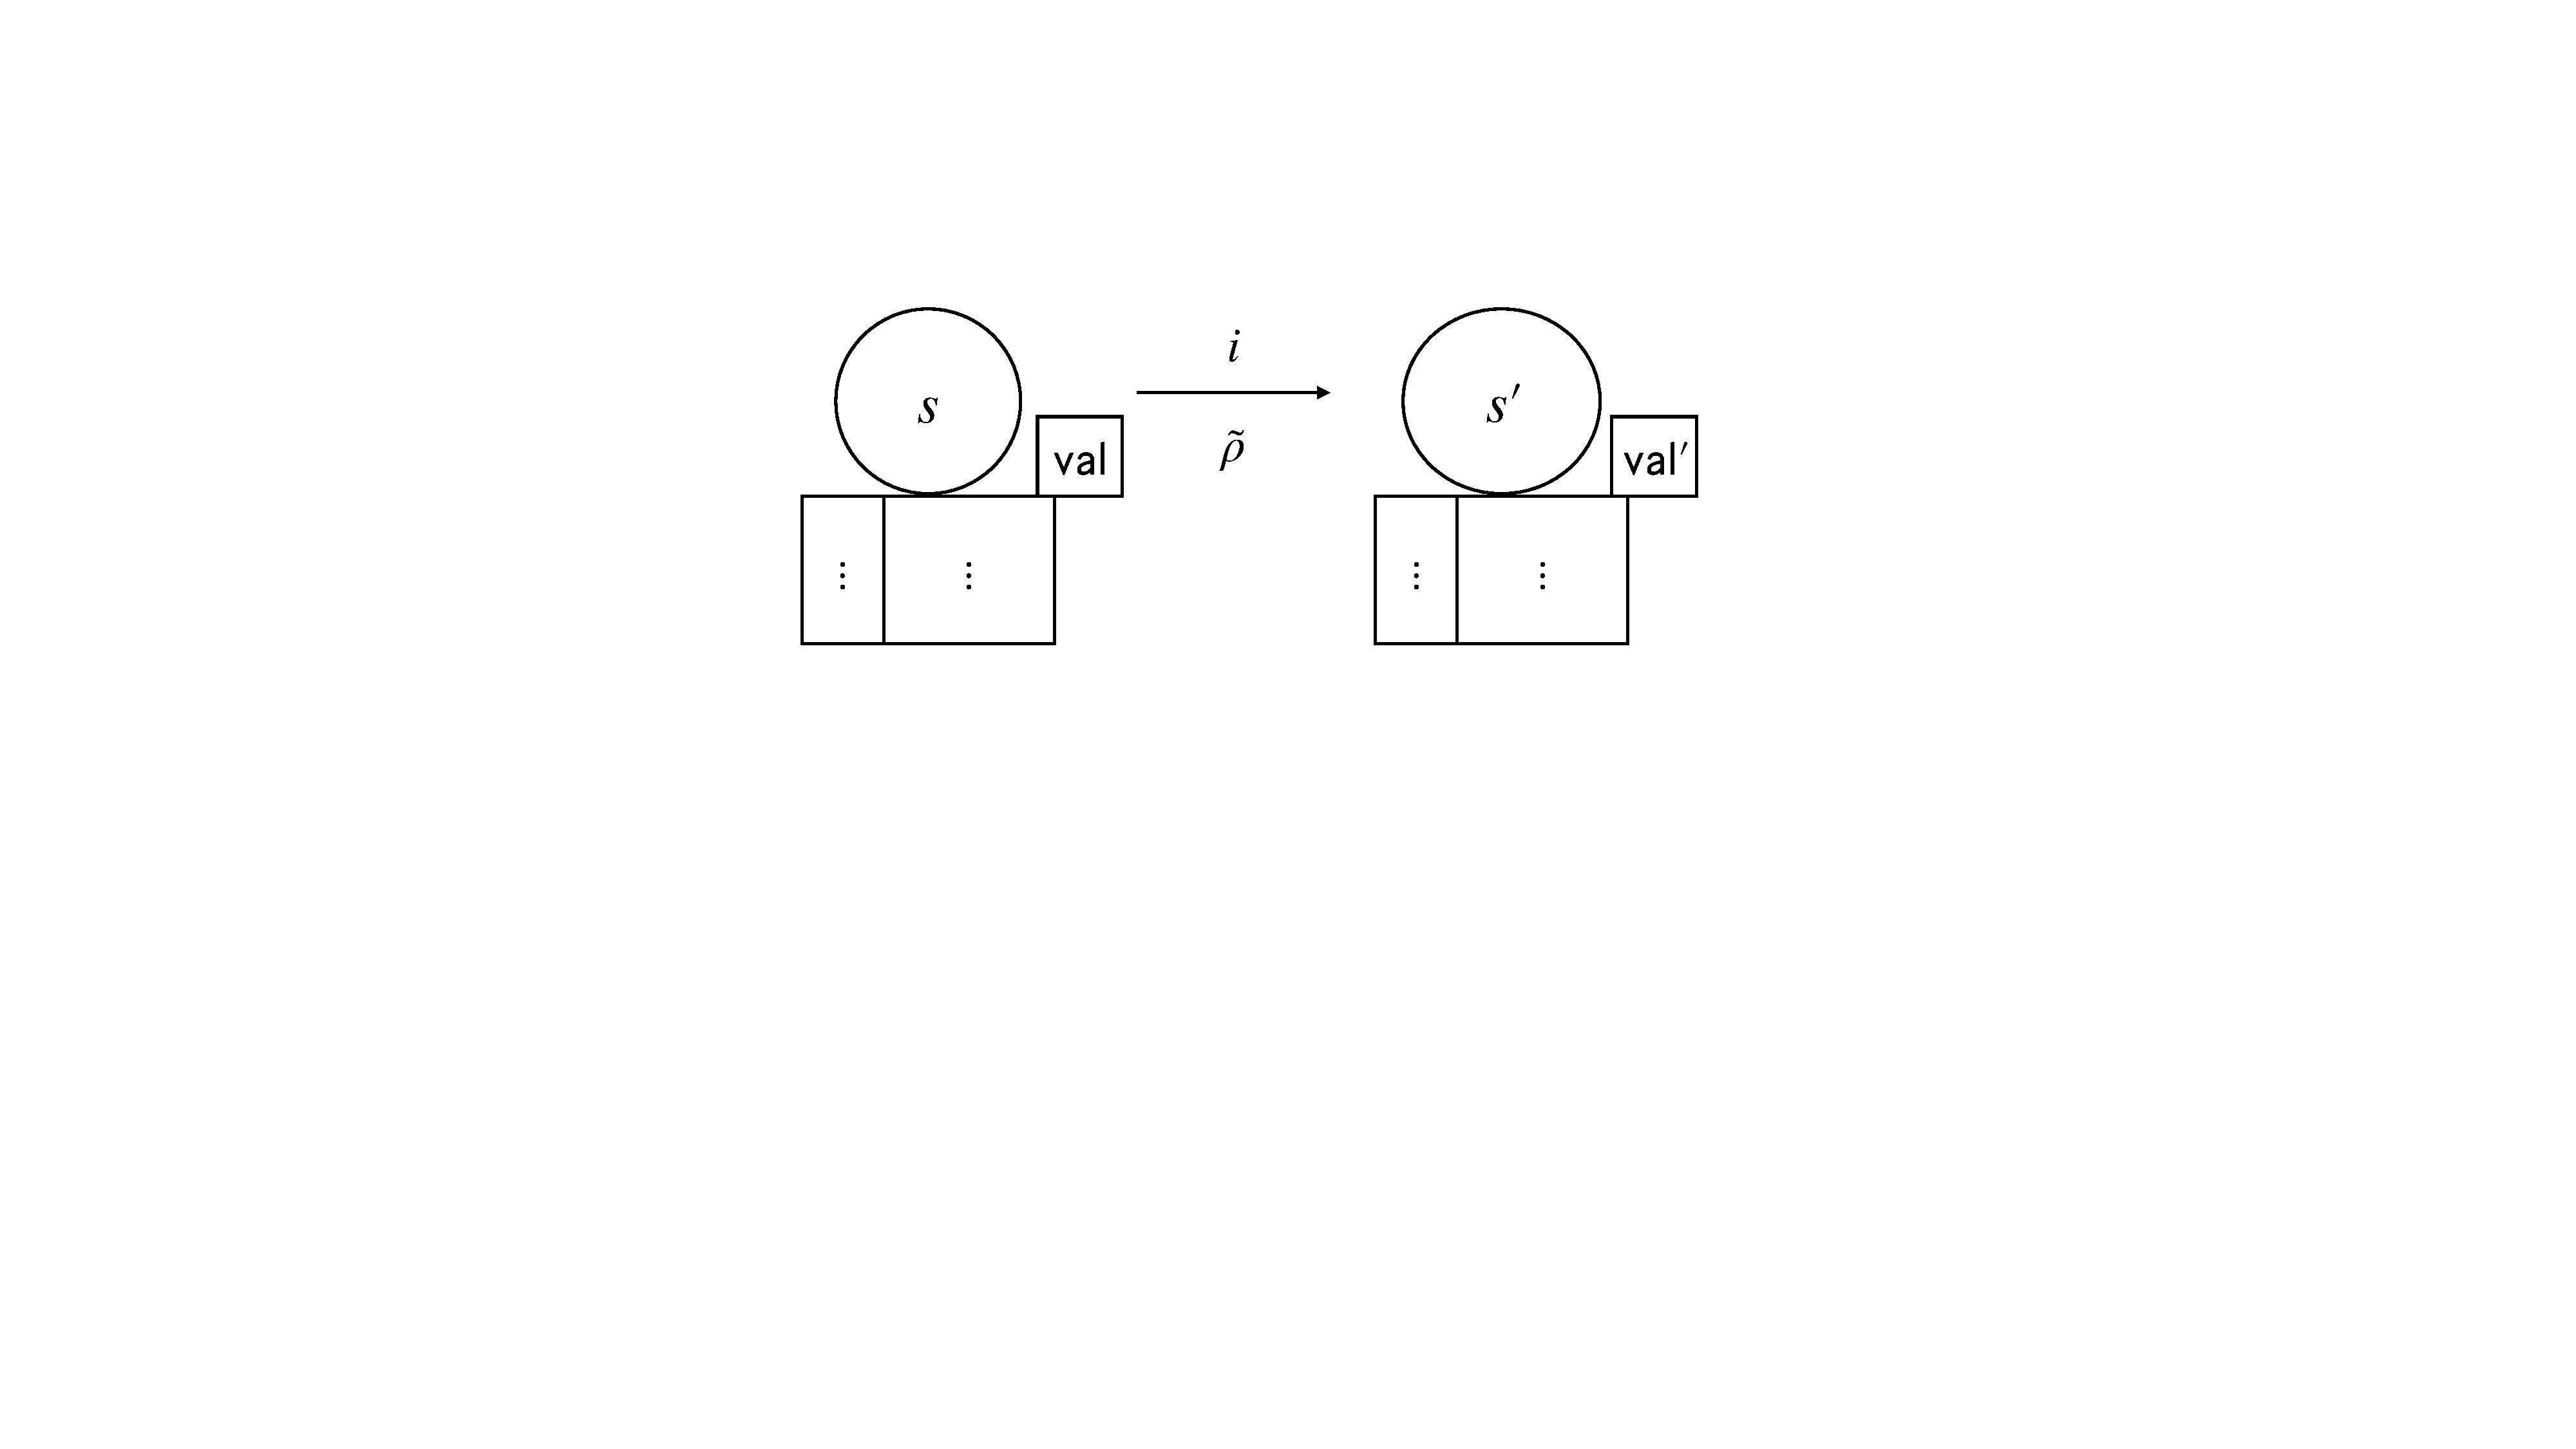
\includegraphics[scale=.2,width=\columnwidth/3*2]{figures/state-transition_cropped.pdf}
  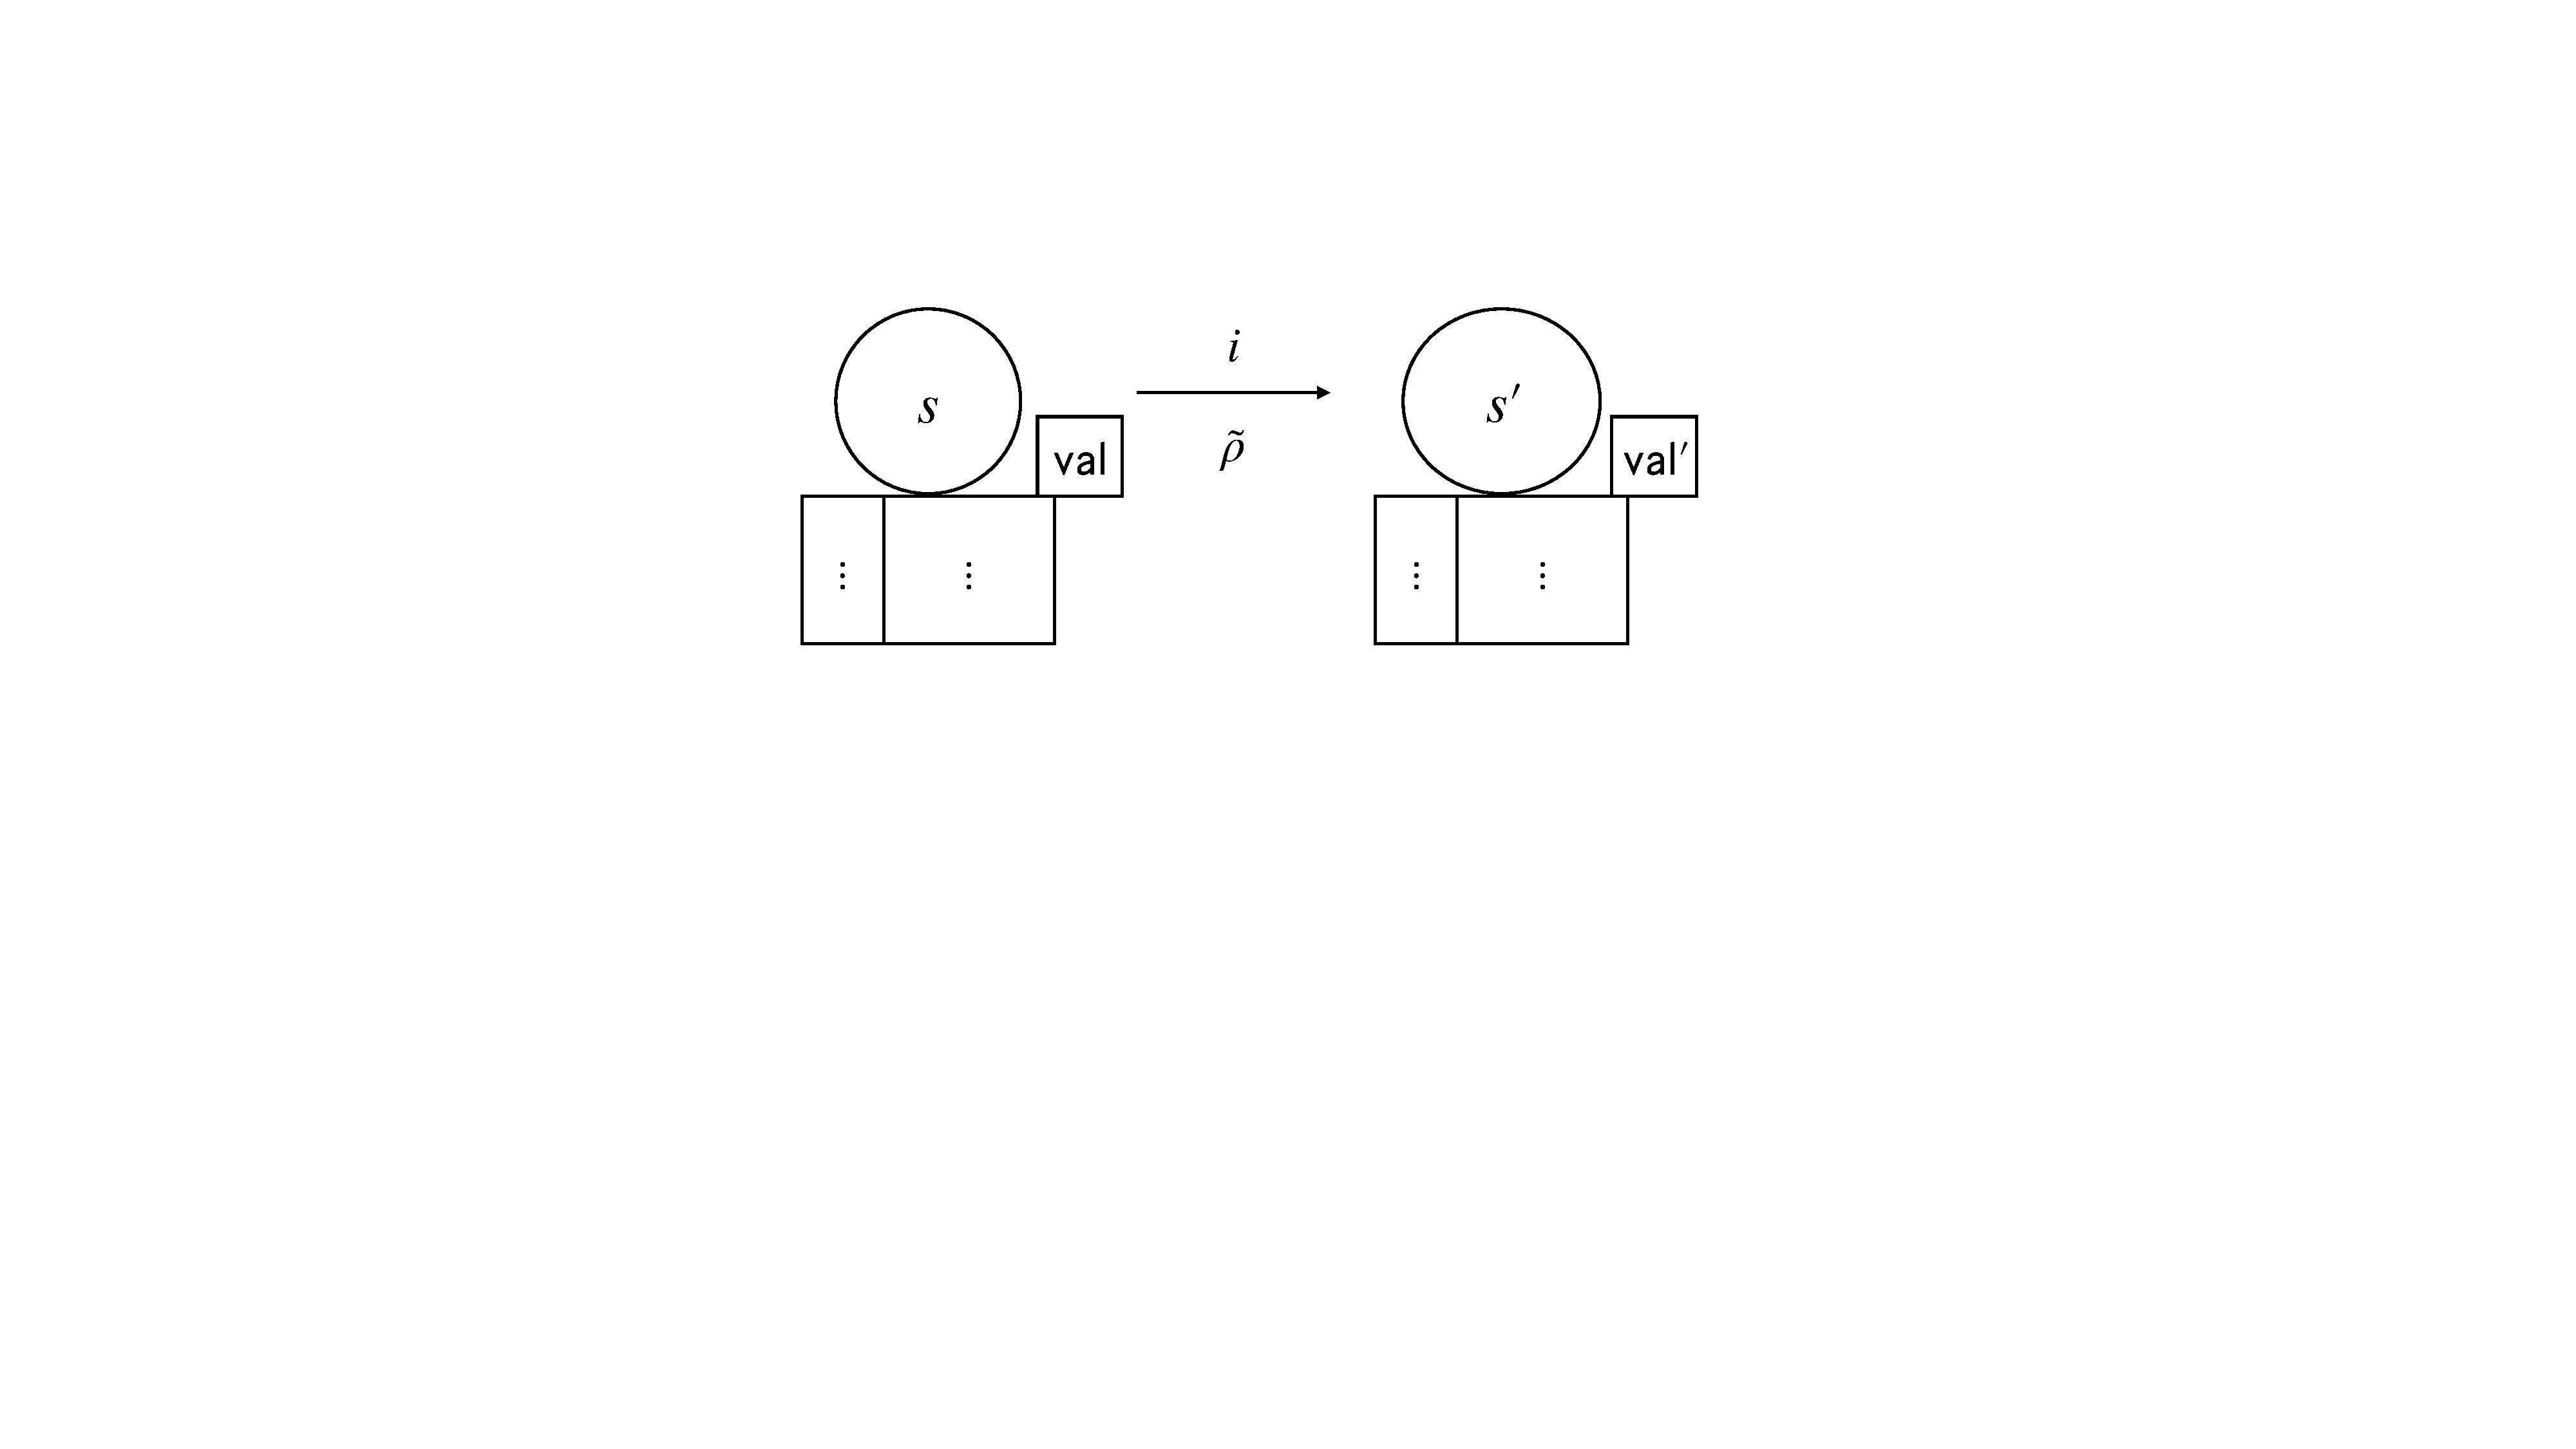
\includegraphics[scale=.2,width=\textwidth/2]{figures/state-transition_cropped.pdf}
  \caption{Transactions representing successive states in a CEM
    transition relation \(\cemStepRel{s}{i}{s'}{\cemTxCon}\).  Fields
    $\val$ and $\val'$ are the value fields of the state-machine
    outputs and $\tilde \rho$ is the additional data.}
  \label{fig:state-transition}
\end{figure}

More specifically, given two transactions $\tx$ and $\tx'$, they represent successive states under \(\cemStepRel{s}{i}{s'}{\cemTxCon}\) iff 
%
\begin{mitemize}
  \item state-machine output $\cemOut = (\txVal, \cemVal, s)$ of $\tx$
  is consumed by the state-machine input $\cemIn' = (\txOutRef, \rho)$
  of $\tx'$, whose redeemer is \(\rho = i\) (i.e., the redeemer
  provides the state-machine input) and
  \item either $\cemFinal(s') = \true$ and $tx'$ has no state-machine
  output, or $\cemOut' = (\txVal', \cemVal, s')$ and $\tx'$ meets all
  constraints imposed by $\cemTxCon$.
\end{mitemize}
Sometimes it is useful to have additional data $\tilde \rho$ provided
as part of the redeemer, i.e., $\rho = (i,\tilde \rho)$.
%
A state transition of the described type is represented by two connected
transactions as shown in Fig.~\ref{fig:state-transition}.  For
simplicity, state-machine inputs and outputs are not shown, with the
exception of the value fields $\txVal$ and $\txVal'$ of the state-machine output.


%%% Local Variables:
%%% mode: latex
%%% TeX-master: "main"
%%% End:
